% ============================================================
%  第 1 周实验报告 — 王本熙 (25020007117)
%  课程: 系统开发工具基础  时间: 2026-08-24 (周一, 第 5—8 节)
%  内容: 课程概览 + Shell 入门; Version Control and Git; LaTeX 文档编辑
%  编译方式: xelatex report1.tex (运行两遍以解析交叉引用)
% ============================================================
\documentclass[a4paper,11pt]{ctexart}

% ---------- 页面布局 ----------
\usepackage[
  top=2.5cm, bottom=2.5cm, left=2.5cm, right=2.5cm,
  headheight=15pt, headsep=0.5cm, footskip=0.8cm
]{geometry}

% ---------- 数学与表格 ----------
\usepackage{amsmath, amssymb}
\usepackage{booktabs}
\usepackage{array}
\usepackage{multirow}

% ---------- 图形与链接 ----------
\usepackage{graphicx}
\usepackage[
  colorlinks=true, linkcolor=blue!70!black,
  citecolor=blue!70!black, urlcolor=teal!80!black
]{hyperref}
\usepackage{xcolor}

% ---------- 代码块 ----------
\usepackage{listings}
\usepackage{subcaption}
\definecolor{codebg}{RGB}{248,248,248}
\definecolor{codekw}{RGB}{0,0,180}
\definecolor{codecmt}{RGB}{0,128,0}
\definecolor{codestr}{RGB}{180,0,0}
\lstset{
  backgroundcolor=\color{codebg},
  basicstyle=\ttfamily\small,
  keywordstyle=\color{codekw}\bfseries,
  commentstyle=\color{codecmt},
  stringstyle=\color{codestr},
  numbers=left, numberstyle=\tiny\color{gray},
  frame=single, rulecolor=\color{gray!40},
  breaklines=true, showstringspaces=false,
  tabsize=2, columns=flexible
}

% ---------- 页眉页脚 ----------
\usepackage{fancyhdr}
\pagestyle{fancy}
\fancyhf{}
\fancyhead[L]{\small 王本熙 \quad 25020007117}
\fancyhead[R]{\small 第 1 周实验报告}
\fancyfoot[C]{\thepage}
\renewcommand{\headrulewidth}{0.4pt}

% ---------- 章节标题样式 ----------
\usepackage{titlesec}
\definecolor{secblue}{RGB}{30,80,160}
\titleformat{\section}
  {\Large\bfseries\color{secblue}}{第\thesection\,章}{0.6em}{}
\titleformat{\subsection}
  {\large\bfseries\color{secblue!80!black}}{\thesubsection}{0.5em}{}
\titleformat{\subsubsection}
  {\normalsize\bfseries\color{secblue!60!black}}{\thesubsubsection}{0.5em}{}

% ---------- 超链接元信息 ----------
\hypersetup{
  pdftitle={第 1 周实验报告},
  pdfauthor={王本熙}
}

% ============================================================
\begin{document}

% ---------- 封面 ----------
\begin{titlepage}
  \centering
  \vspace*{2cm}
  {\Huge\bfseries\color{secblue} 实验报告\par}
  \vspace{0.8cm}
  {\Large 第 1 周：Shell 入门 · Git · LaTeX\par}
  \vspace{3cm}
  \begin{tabular}{rl}
    \Large 姓\quad 名\,:\, & \Large 王本熙 \\[0.8em]
    \Large 学\quad 号\,:\, & \Large 25020007117 \\[0.8em]
    \Large 日\quad 期\,:\, & \Large 2026 年 8 月 24 日 \\[0.8em]
    \Large 平\quad 台\,:\, & \Large Windows + WSL (Ubuntu) \\
  \end{tabular}
  \vfill
  \rule{10cm}{0.4pt}
  \vspace*{1cm}
\end{titlepage}

% ---------- 目录 ----------
\tableofcontents
\newpage

% ============================================================
\section{实验目的}

本实验为课程第 1 周的课上实验检查题，旨在掌握以下内容：
\begin{itemize}
  \item Shell 基础与文件系统操作：正确创建、复制含空格文件名的文件，
        并管理目录与文件权限；
  \item Shell 管道与文本处理：使用 awk、sort、head 等工具完成日志统计，
        并规范处理标准错误流与非零退出码；
  \item Version Control and Git：主动制造并解决一次合并冲突，
        理解冲突产生的原因与解决流程；
  \item \LaTeX{} 文档编辑：加入带编号公式与表格并交叉引用，
        从命令行构建 PDF 且引用不显示 \texttt{??}。
\end{itemize}

各题内容概览如表~\ref{tab:overview} 所示。

\begin{table}[htbp]
  \centering
  \caption{第 1 周实验内容概览}\label{tab:overview}
  \begin{tabular}{clcl}
    \toprule
    题号 & 主题 & 关键工具 & 成果 \\
    \midrule
    1 & 含空格文件名的批量整理 & mkdir / cp / find / chmod & work 目录与 inventory.txt \\
    2 & 随机访问日志统计 & 管道 / awk / sort / head & analyze.sh \\
    3 & 制造、解决并解释合并冲突 & git branch / merge & 冲突解决与提交历史 \\
    4 & 修复并构建一页技术说明 & \LaTeX{} / xelatex & report.pdf \\
    \bottomrule
  \end{tabular}
\end{table}

% ============================================================
\section{实验环境}

\begin{table}[htbp]
  \centering
  \caption{实验环境}\label{tab:env}
  \begin{tabular}{ll}
    \toprule
    项目 & 配置 \\
    \midrule
    操作系统 & Windows + WSL (Ubuntu) \\
    编辑器 & VS Code / Trae IDE \\
    Shell 与工具链 & bash, coreutils, find, awk, sort, head \\
    版本管理 & Git \\
    排版引擎 & XeLaTeX（ctexart 文档类） \\
    \bottomrule
  \end{tabular}
\end{table}

% ============================================================
\section{第 1 题：含空格文件名的批量整理}

\subsection{任务描述}

在当前目录新建 \texttt{q01}，完全使用命令行完成：创建含空格文件名、
隐藏文件与空文件的测试文件；显示绝对路径并以长格式列出全部项目
（含隐藏文件）；将所有 \texttt{.txt} 文件复制到 \texttt{work/<学号>}/
并保留相对目录结构；设置目录权限 750、文件权限 640；
生成含相对路径与字节数的清单 \texttt{inventory.txt}。

\subsection{命令实现}

关键在于：文件名含空格时用双引号包裹；复制阶段采用
\textbf{\texttt{rsync}} 的 \texttt{--include} / \texttt{--exclude}
规则，在保留目录结构的同时精准收齐所有 \texttt{.txt}
（包括隐藏的 \texttt{.secret.txt}），无需手动遍历。

\begin{lstlisting}[language=bash]
# 1. 创建目录与测试文件(含空格文件名、隐藏文件、空文件)
mkdir -p q01/{docs,tmp}
echo -e "alpha\nbeta"           > "q01/input/docs/notes one.txt"
echo "hidden"                  >  q01/input/docs/.secret.txt
touch q01/input/tmp/empty.txt
echo -e "2026-08-27 10:00:01 用户登录成功\n2026-08-27 10:00:05 请求处理完成" \
  > q01/input/run.log

# 2. 显示绝对路径, 长格式列出 input 全部项目(含隐藏文件)
realpath q01                      # /home/.../q01
ls -la q01/input                  # 顶层
ls -la q01/input/                 # 同上, 效果一致
ls -laR q01/input/                # 递归, 含各子目录

# 3. 复制所有 .txt 到 work/<学号>/, 保留相对目录结构
mkdir -p work/25020007117
rsync -av \
  --include='*/'   \              # 包含所有子目录(递归)
  --include='*.txt' \              # 包含所有 .txt(含隐藏)
  --exclude='*'    \              # 排除其余文件
  q01/input/ work/25020007117/

# 4. 目录 750 / 文件 640, 生成清单(相对路径 + 字节数, 不含清单自身)
find work/25020007117 -type d -exec chmod 750 {} \;
find work/25020007117 -type f -exec chmod 640 {} \;
find work/25020007117 -type f -not -name "inventory.txt" \
  -printf '%P %s\n' | sort > work/25020007117/inventory.txt

# 5. 查看结果
tree work/25020007117             # 目录树
ls -lR work/25020007117           # 确认权限
batcat work/25020007117/inventory.txt  # 清单内容
\end{lstlisting}

\subsection{运行结果}

复制后 \texttt{work/25020007117/} 下保留了
\texttt{docs/notes one.txt}（空格文件名）、
\texttt{docs/.secret.txt}（隐藏文件）与
\texttt{tmp/empty.txt}（空文件）的相对结构；
目录权限均为 \texttt{drwxr-x---}（750）、
文件权限均为 \texttt{-rw-r-----}（640）。
\texttt{inventory.txt} 逐行列出相对路径与字节数，
三行分别为 \texttt{docs/notes one.txt 11}、
\texttt{docs/.secret.txt 7}、\texttt{tmp/empty.txt 0}。
完整过程如图~\ref{fig:q01} 所示。

\begin{figure}[htbp]
  \centering
  \begin{subfigure}[b]{0.98\textwidth}
    \centering
    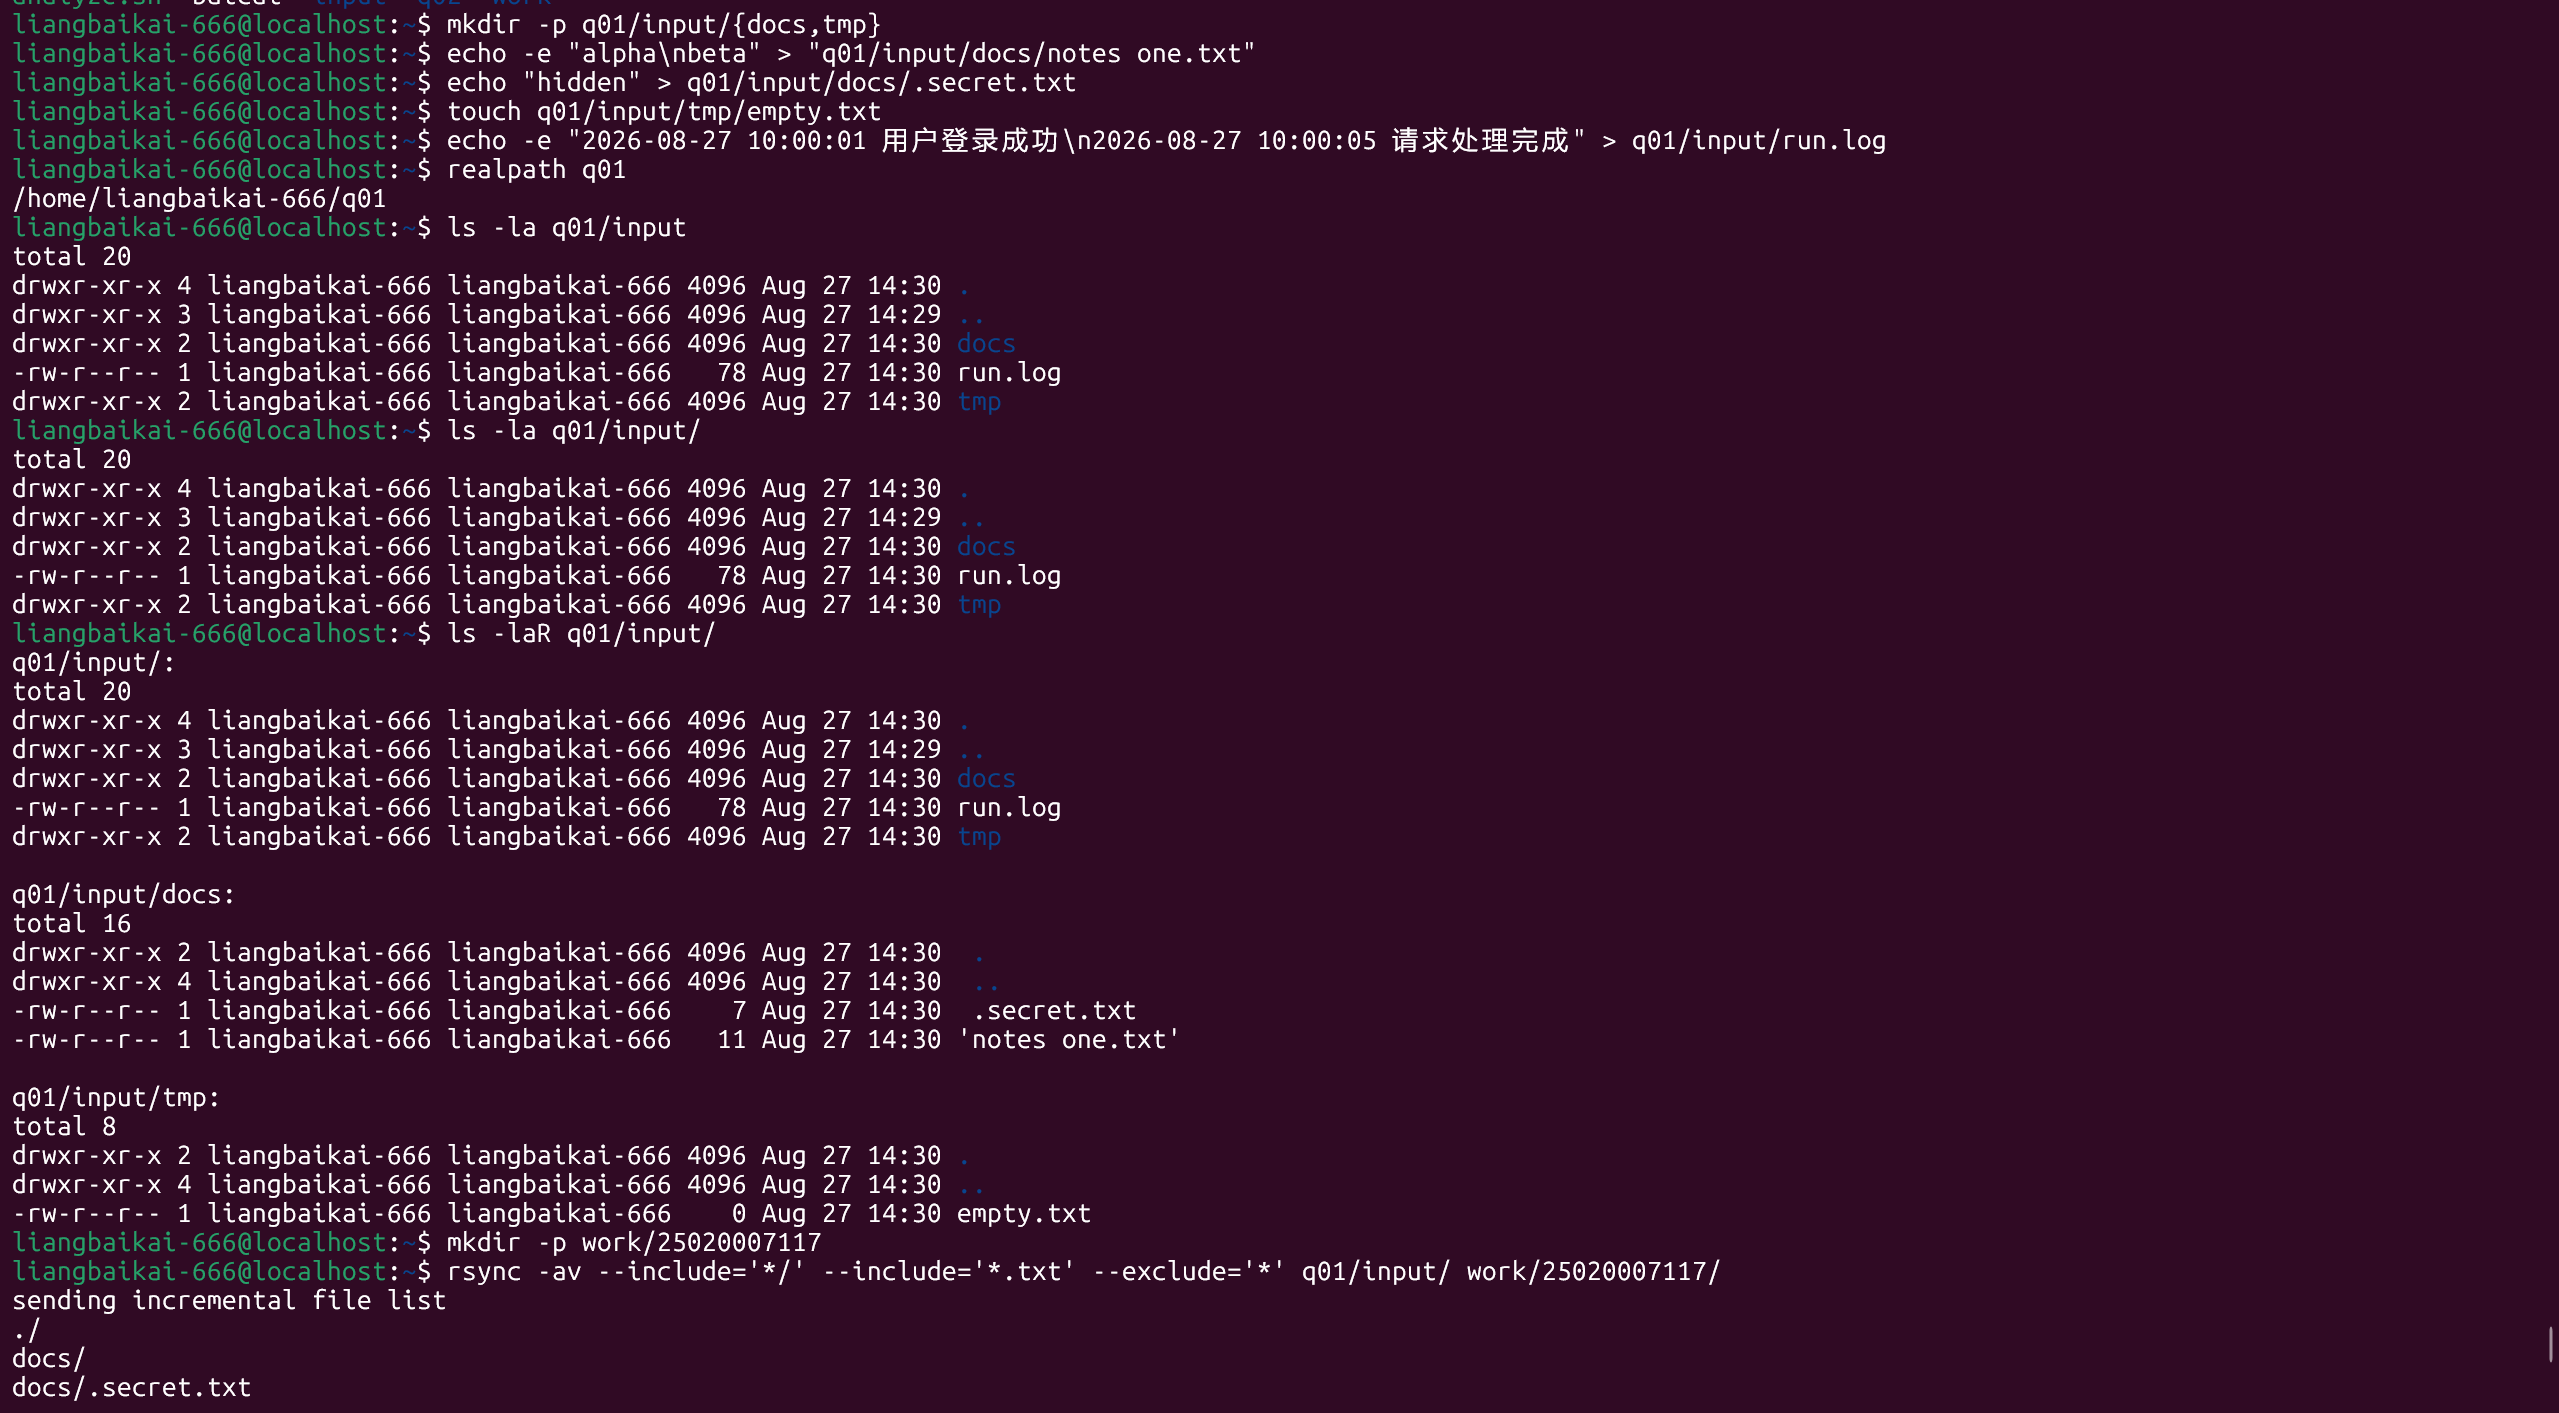
\includegraphics[width=\textwidth]{q01-1.png}
    \caption{创建测试文件 + \texttt{realpath q01} + \texttt{ls -laR q01/input/}}
  \end{subfigure}
  \vspace{0.4em}
  \begin{subfigure}[b]{0.98\textwidth}
    \centering
    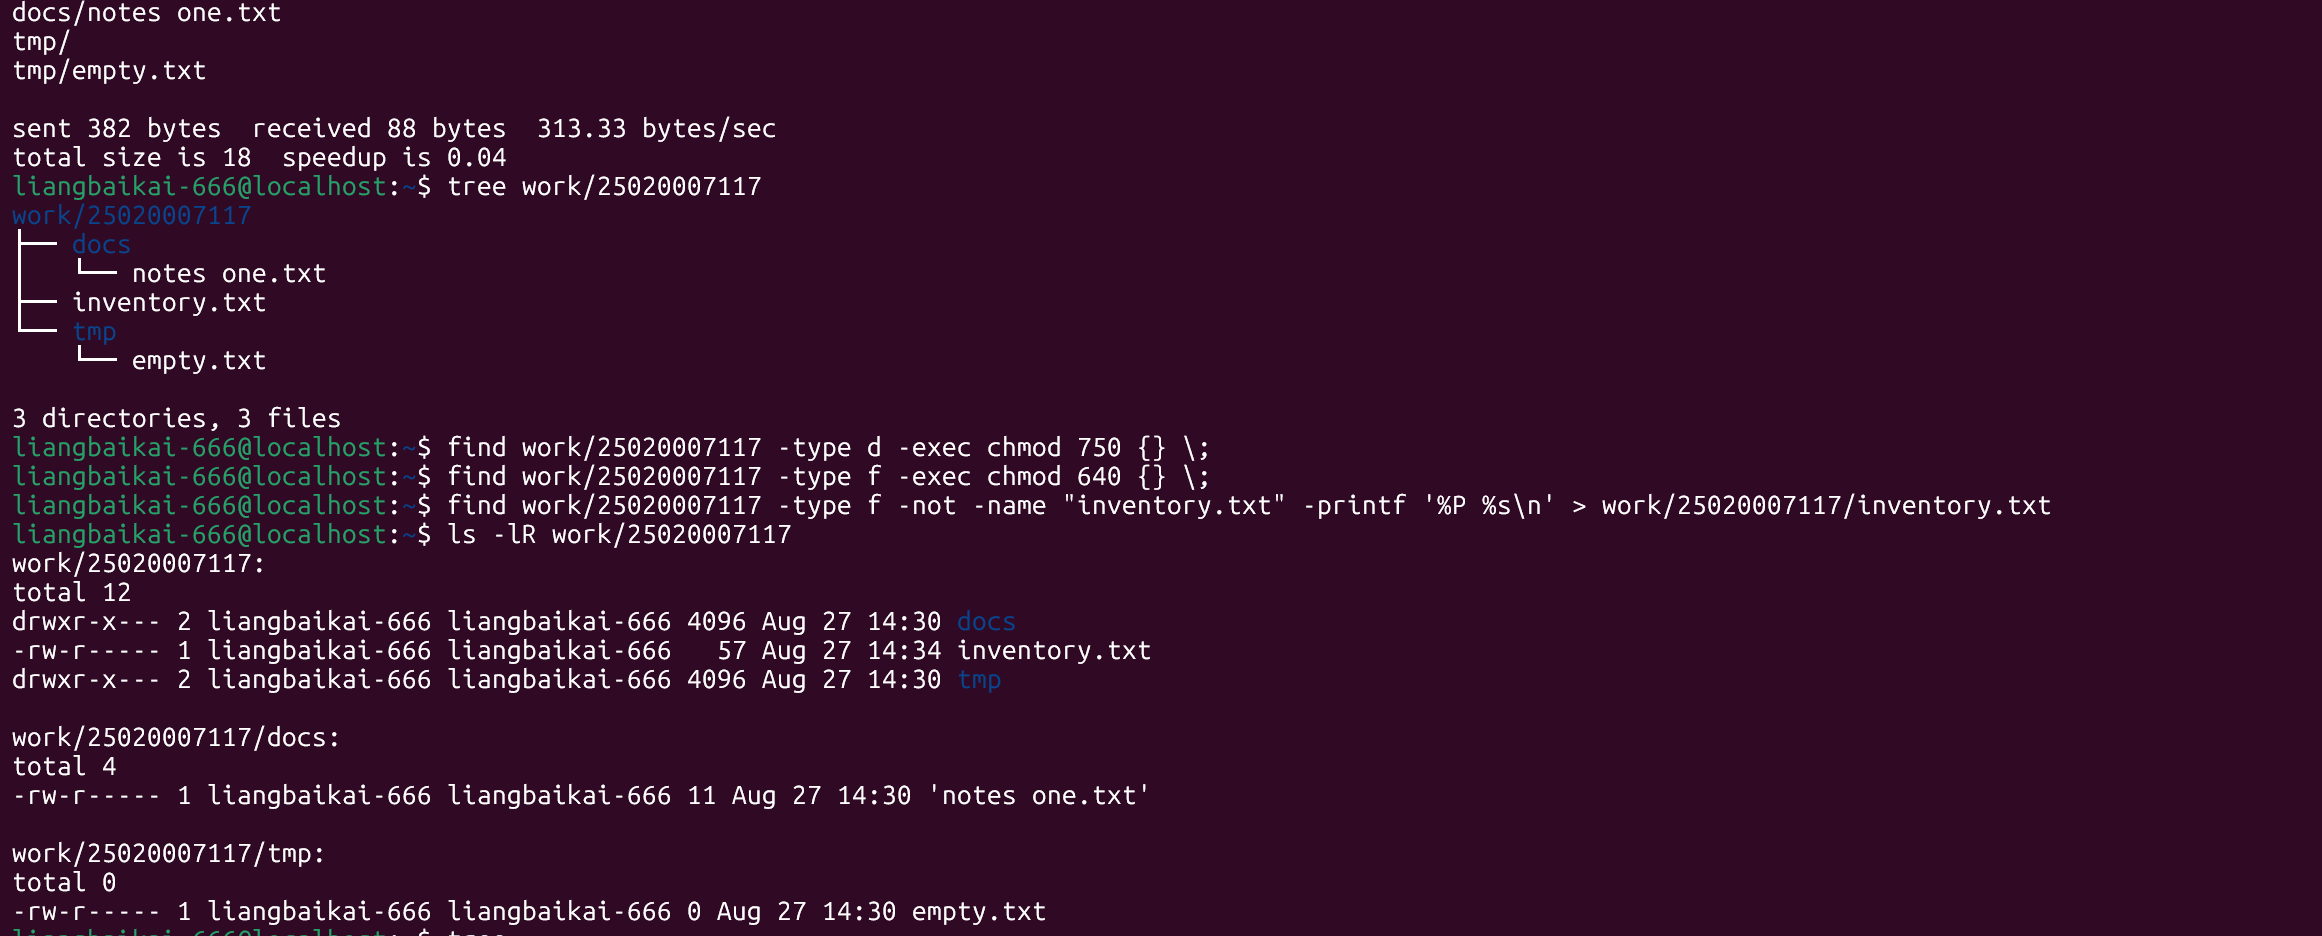
\includegraphics[width=\textwidth]{q01-2.png}
    \caption{\texttt{rsync} 复制 + \texttt{tree} 查看目录结构 + \texttt{chmod} + \texttt{ls -lR} 确认权限}
  \end{subfigure}
  \vspace{0.4em}
  \begin{subfigure}[b]{0.98\textwidth}
    \centering
    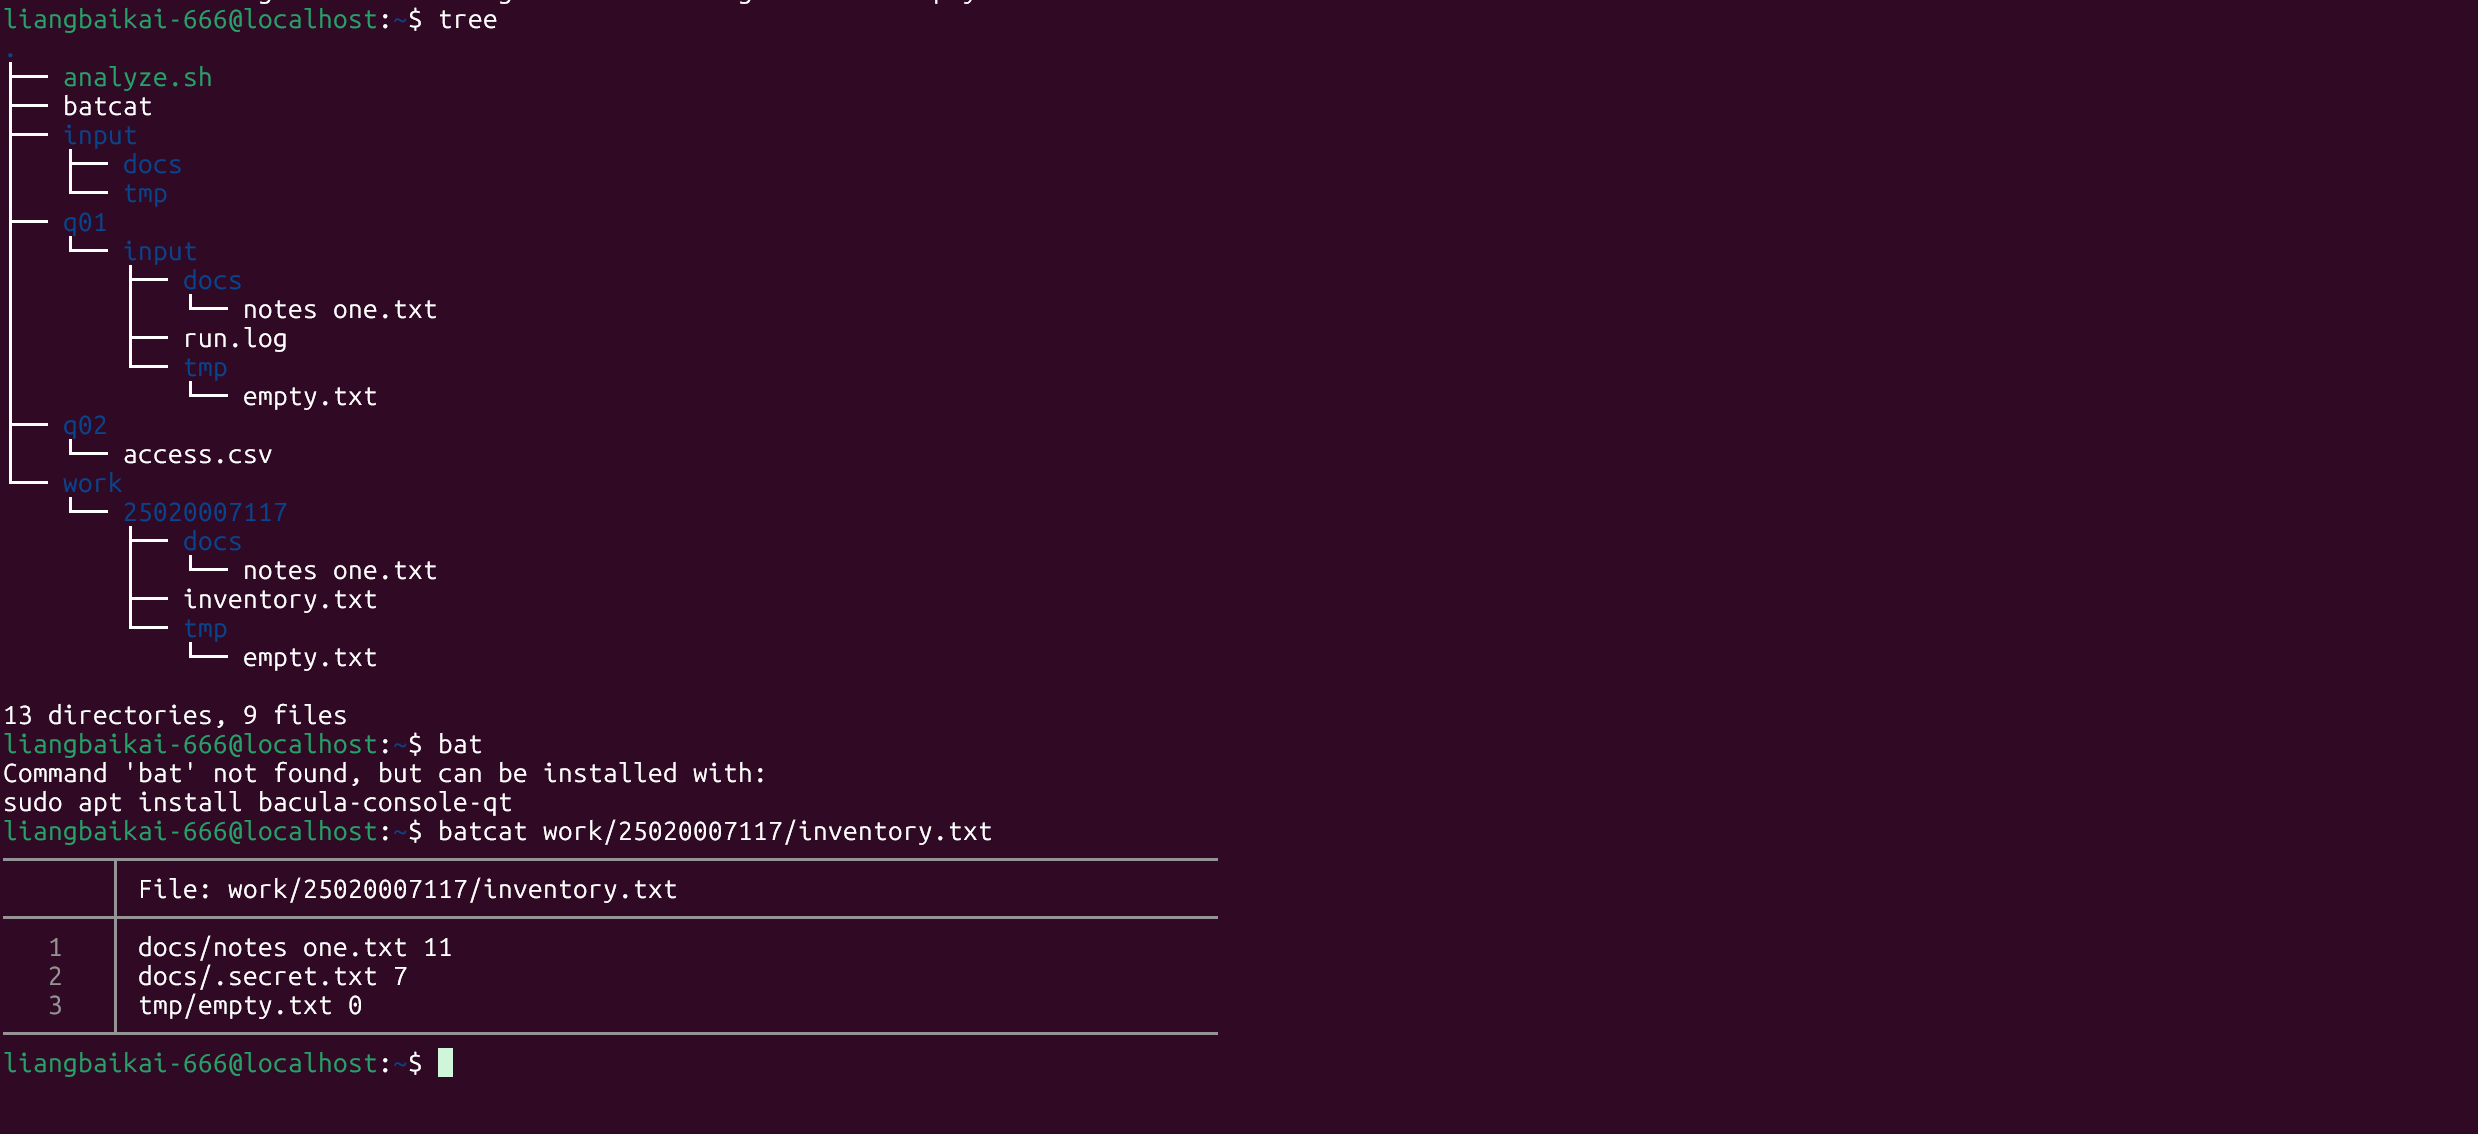
\includegraphics[width=\textwidth]{q01-3.png}
    \caption{整体目录树 + \texttt{batcat} 查看 \texttt{inventory.txt}}
  \end{subfigure}
  \caption{第 1 题：含空格文件名的批量整理全过程截图}
  \label{fig:q01}
\end{figure}

% ============================================================
\section{第 2 题：随机访问日志统计}

\subsection{脚本实现}

编写 \texttt{analyze.sh}，接收一个 CSV 文件路径；无参数时提示用法、
文件不存在时将错误写入 stderr，均返回非零退出码。
统计部分使用管道串联 \texttt{tail}、\texttt{awk}、\texttt{sort}、
\texttt{uniq -c}、\texttt{head} 完成，全程未使用 Python、
电子表格或手工统计。脚本经历多次迭代调试（见图~\ref{fig:q02}b），
最终版本如下：

\begin{lstlisting}[language=bash]
#!/bin/bash
# analyze.sh — 统计 5xx 最多的前 2 个 path 与平均 latency_ms

# 1. 参数检查: 无参数则 stderr 提示并退出
if [ $# -eq 0 ]; then
    echo "error:please give a path of .csv as augument">&2
    exit 1
fi

# 2. 文件存在性检查
csv_file="$1"
if test ! -f "$csv_file" ; then
   echo "error:file '$csv_file'not exist." >&2
   exit 1
fi

# 3) 5xx 次数最多的前 2 个 path (次数降序, 相同按 path 字典序)
echo "=== HTTP 5xx nums  1st and 2ed of paths ==="
tail -n +2 "$csv_file"          |   # 跳过表头
awk -F, '$4 >= 500 && $4 < 600 {print $3}' |   # 筛选 5xx, 输出 path
sort | uniq -c                  |   # 计数
sort -k1,1nr -k2,2              |   # 次数降序, 同则 path 升序
head -n 2

echo " "

# 4) 全部数据行的平均 latency_ms (跳过表头, 保留两位小数)
echo "=== all average latency_ms of data lines ==="
tail -n +2 "$csv_file"          |
awk -F, '{ sum += $5; count++ } END { printf "%.2f\n", sum / count }'
\end{lstlisting}

\subsection{运行结果}

对 \texttt{access.csv} 运行，得到 5xx 最多的前 2 个 path 与平均延迟；
对不存在的文件运行时错误写入 stderr 且退出码非零：

\begin{lstlisting}[numbers=none]
$ ./analyze.sh access.csv
=== HTTP 5xx nums  1st and 2ed of paths ===
   3 /api/orders
   2 /api/users

=== all average latency_ms of data lines ===
193.75

$ ./analyze.sh missing.csv
error:file 'missing.csv'not exist.
\end{lstlisting}

其中 \texttt{tail -n +2} 跳过表头行，保证表头不计入平均延迟；
5 条 5xx 分布在 \texttt{/api/orders}（3 次）、
\texttt{/api/users}（2 次）、\texttt{/login}（1 次），
按次数降序、同则 path 字典序排列后前 2 名与预期一致。
8 条数据行的 latency 总和为 1550 ms，平均为 193.75 ms。

完整过程如图~\ref{fig:q02} 所示。

\begin{figure}[htbp]
  \centering
  \begin{subfigure}[b]{0.98\textwidth}
    \centering
    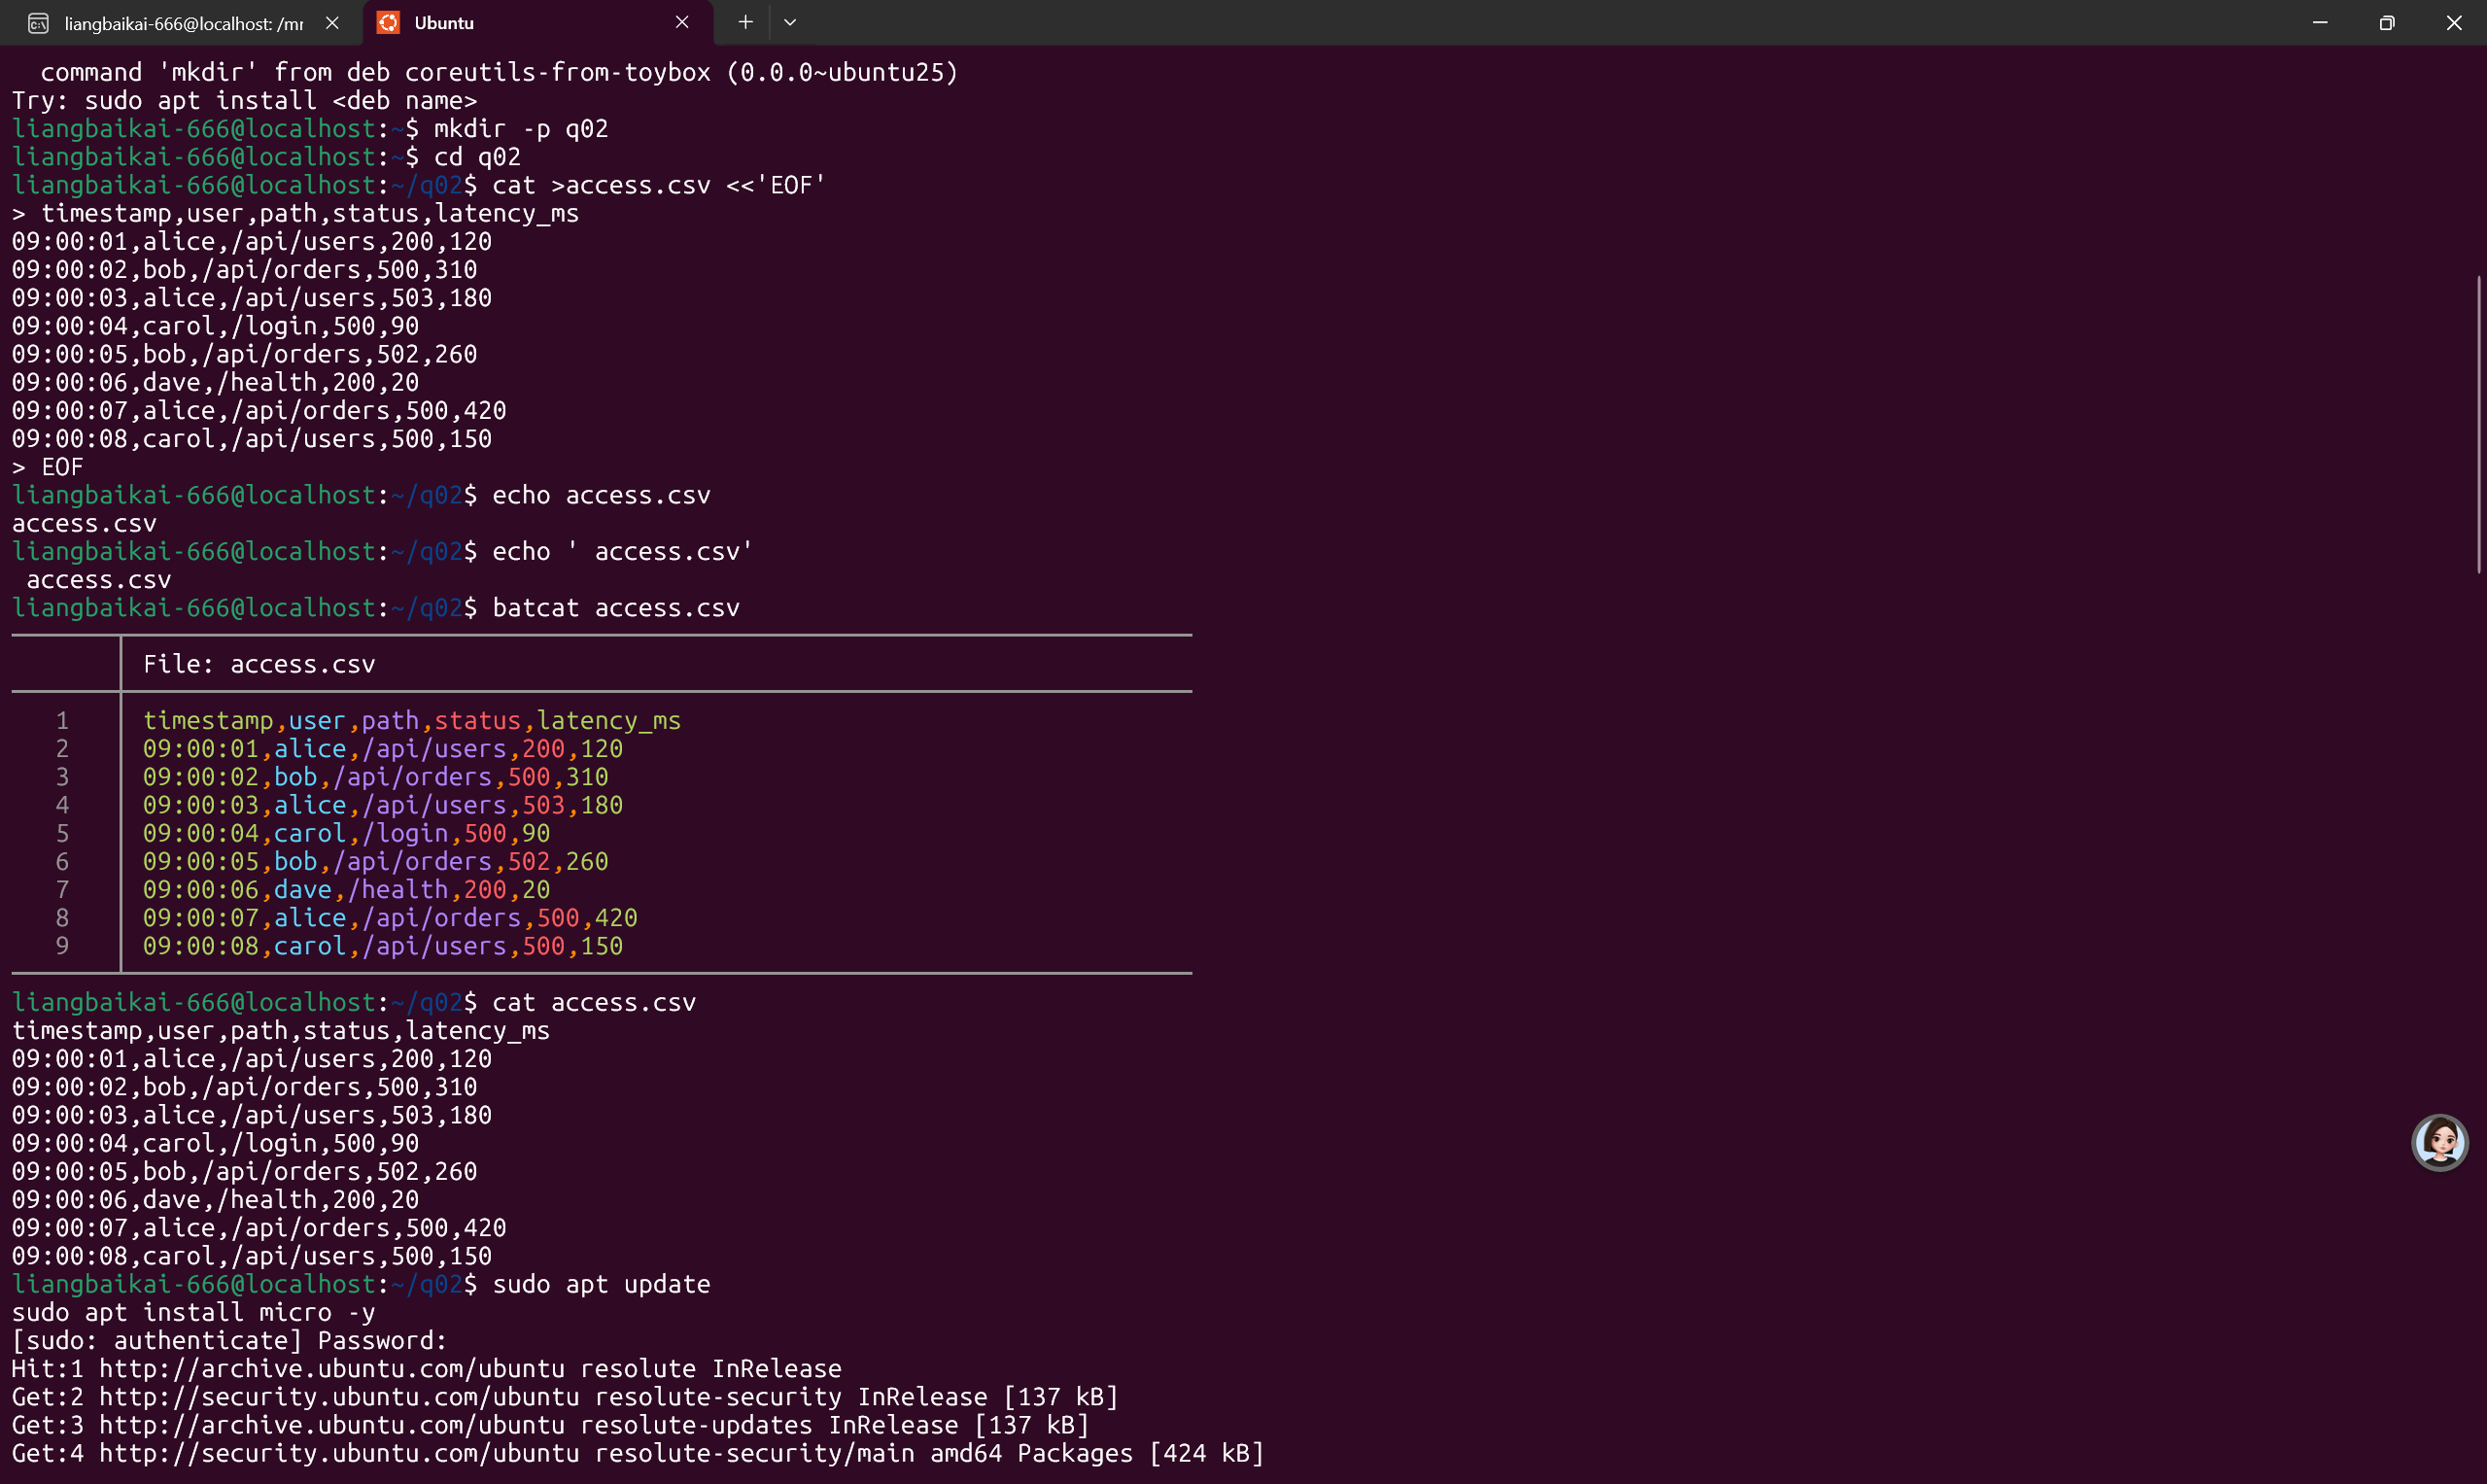
\includegraphics[width=\textwidth]{q02-1.png}
    \caption{创建 \texttt{access.csv}（heredoc）+ \texttt{batcat} 查看内容}
    \label{fig:q02a}
  \end{subfigure}
  \vspace{0.4em}
  \begin{subfigure}[b]{0.98\textwidth}
    \centering
    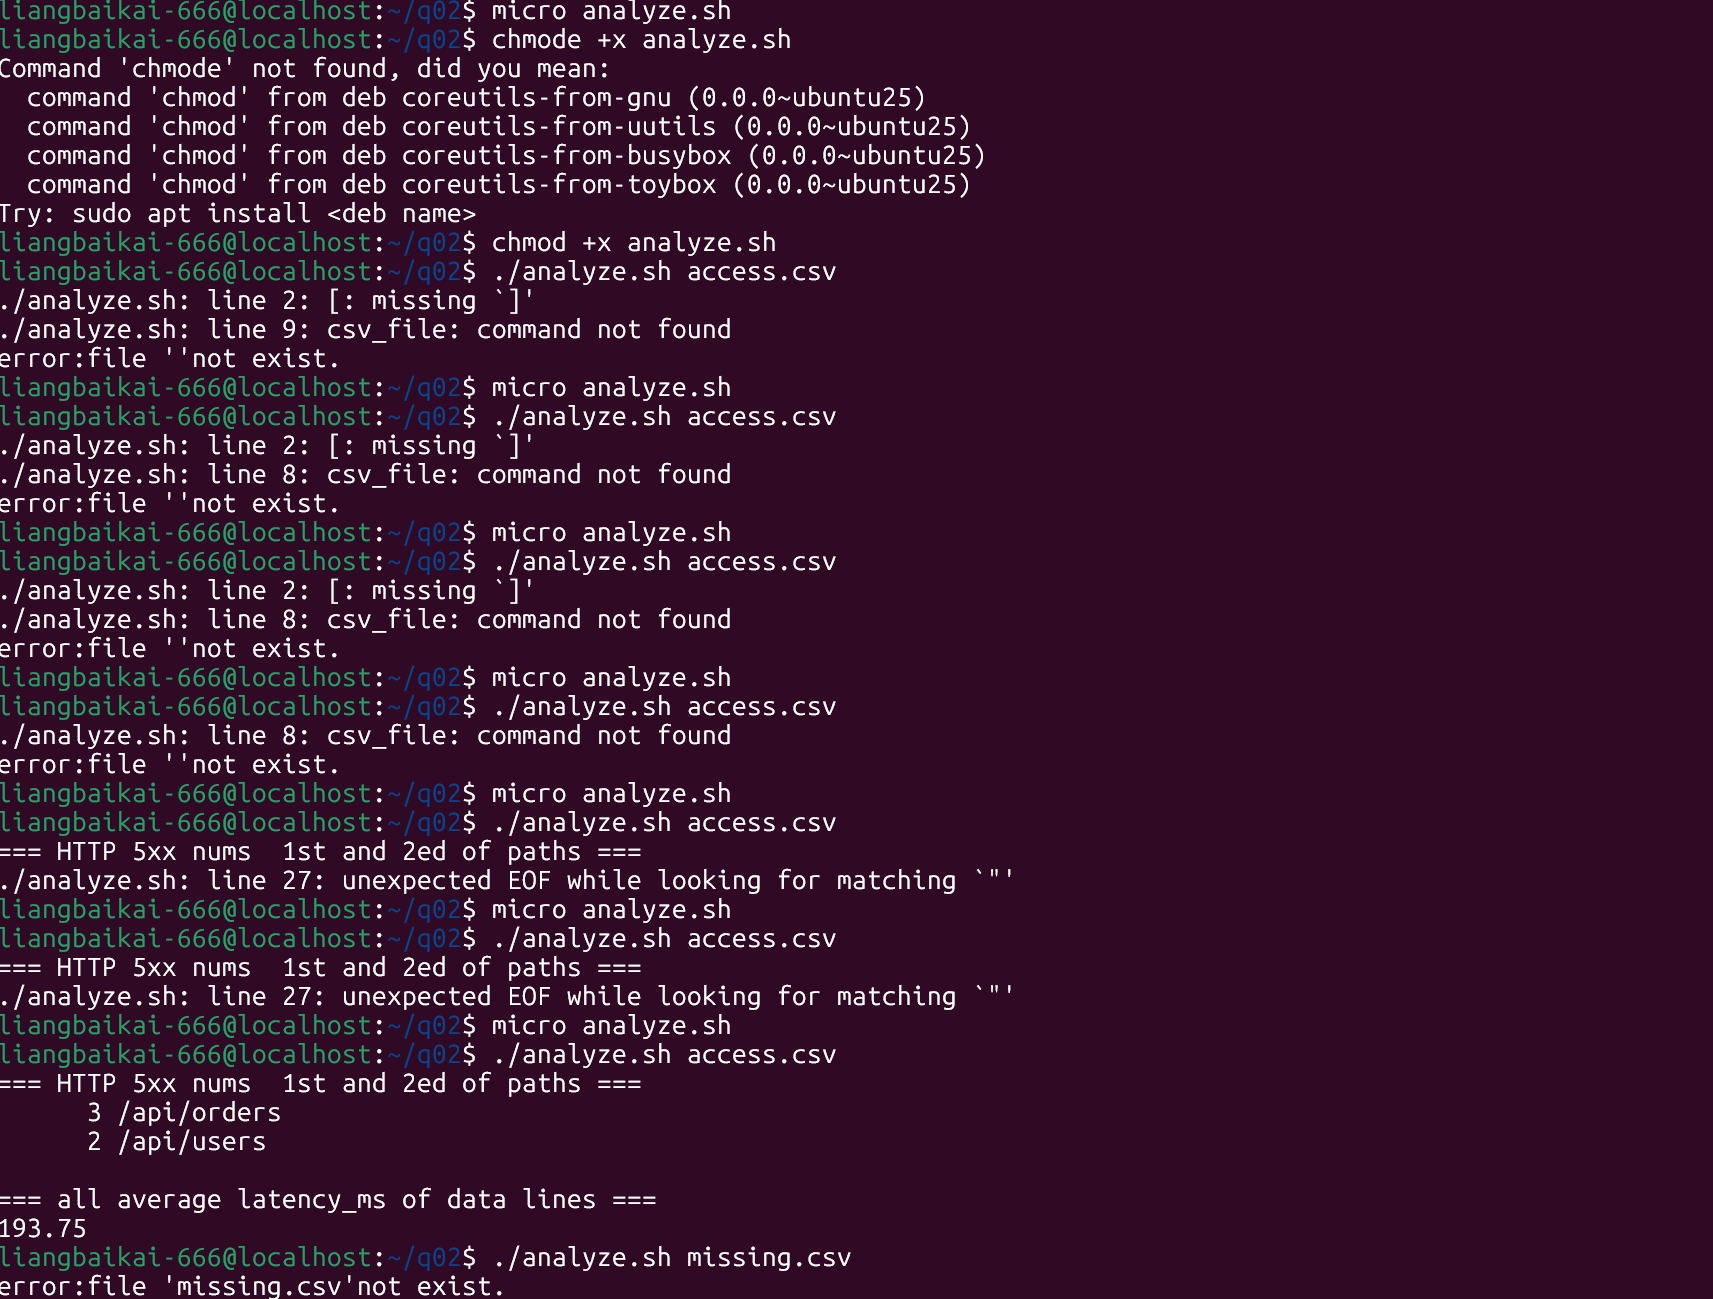
\includegraphics[width=\textwidth]{q02-2.png}
    \caption{脚本迭代调试过程 + 最终运行结果（含对不存在文件的错误输出）}
    \label{fig:q02b}
  \end{subfigure}
  \vspace{0.4em}
  \begin{subfigure}[b]{0.98\textwidth}
    \centering
    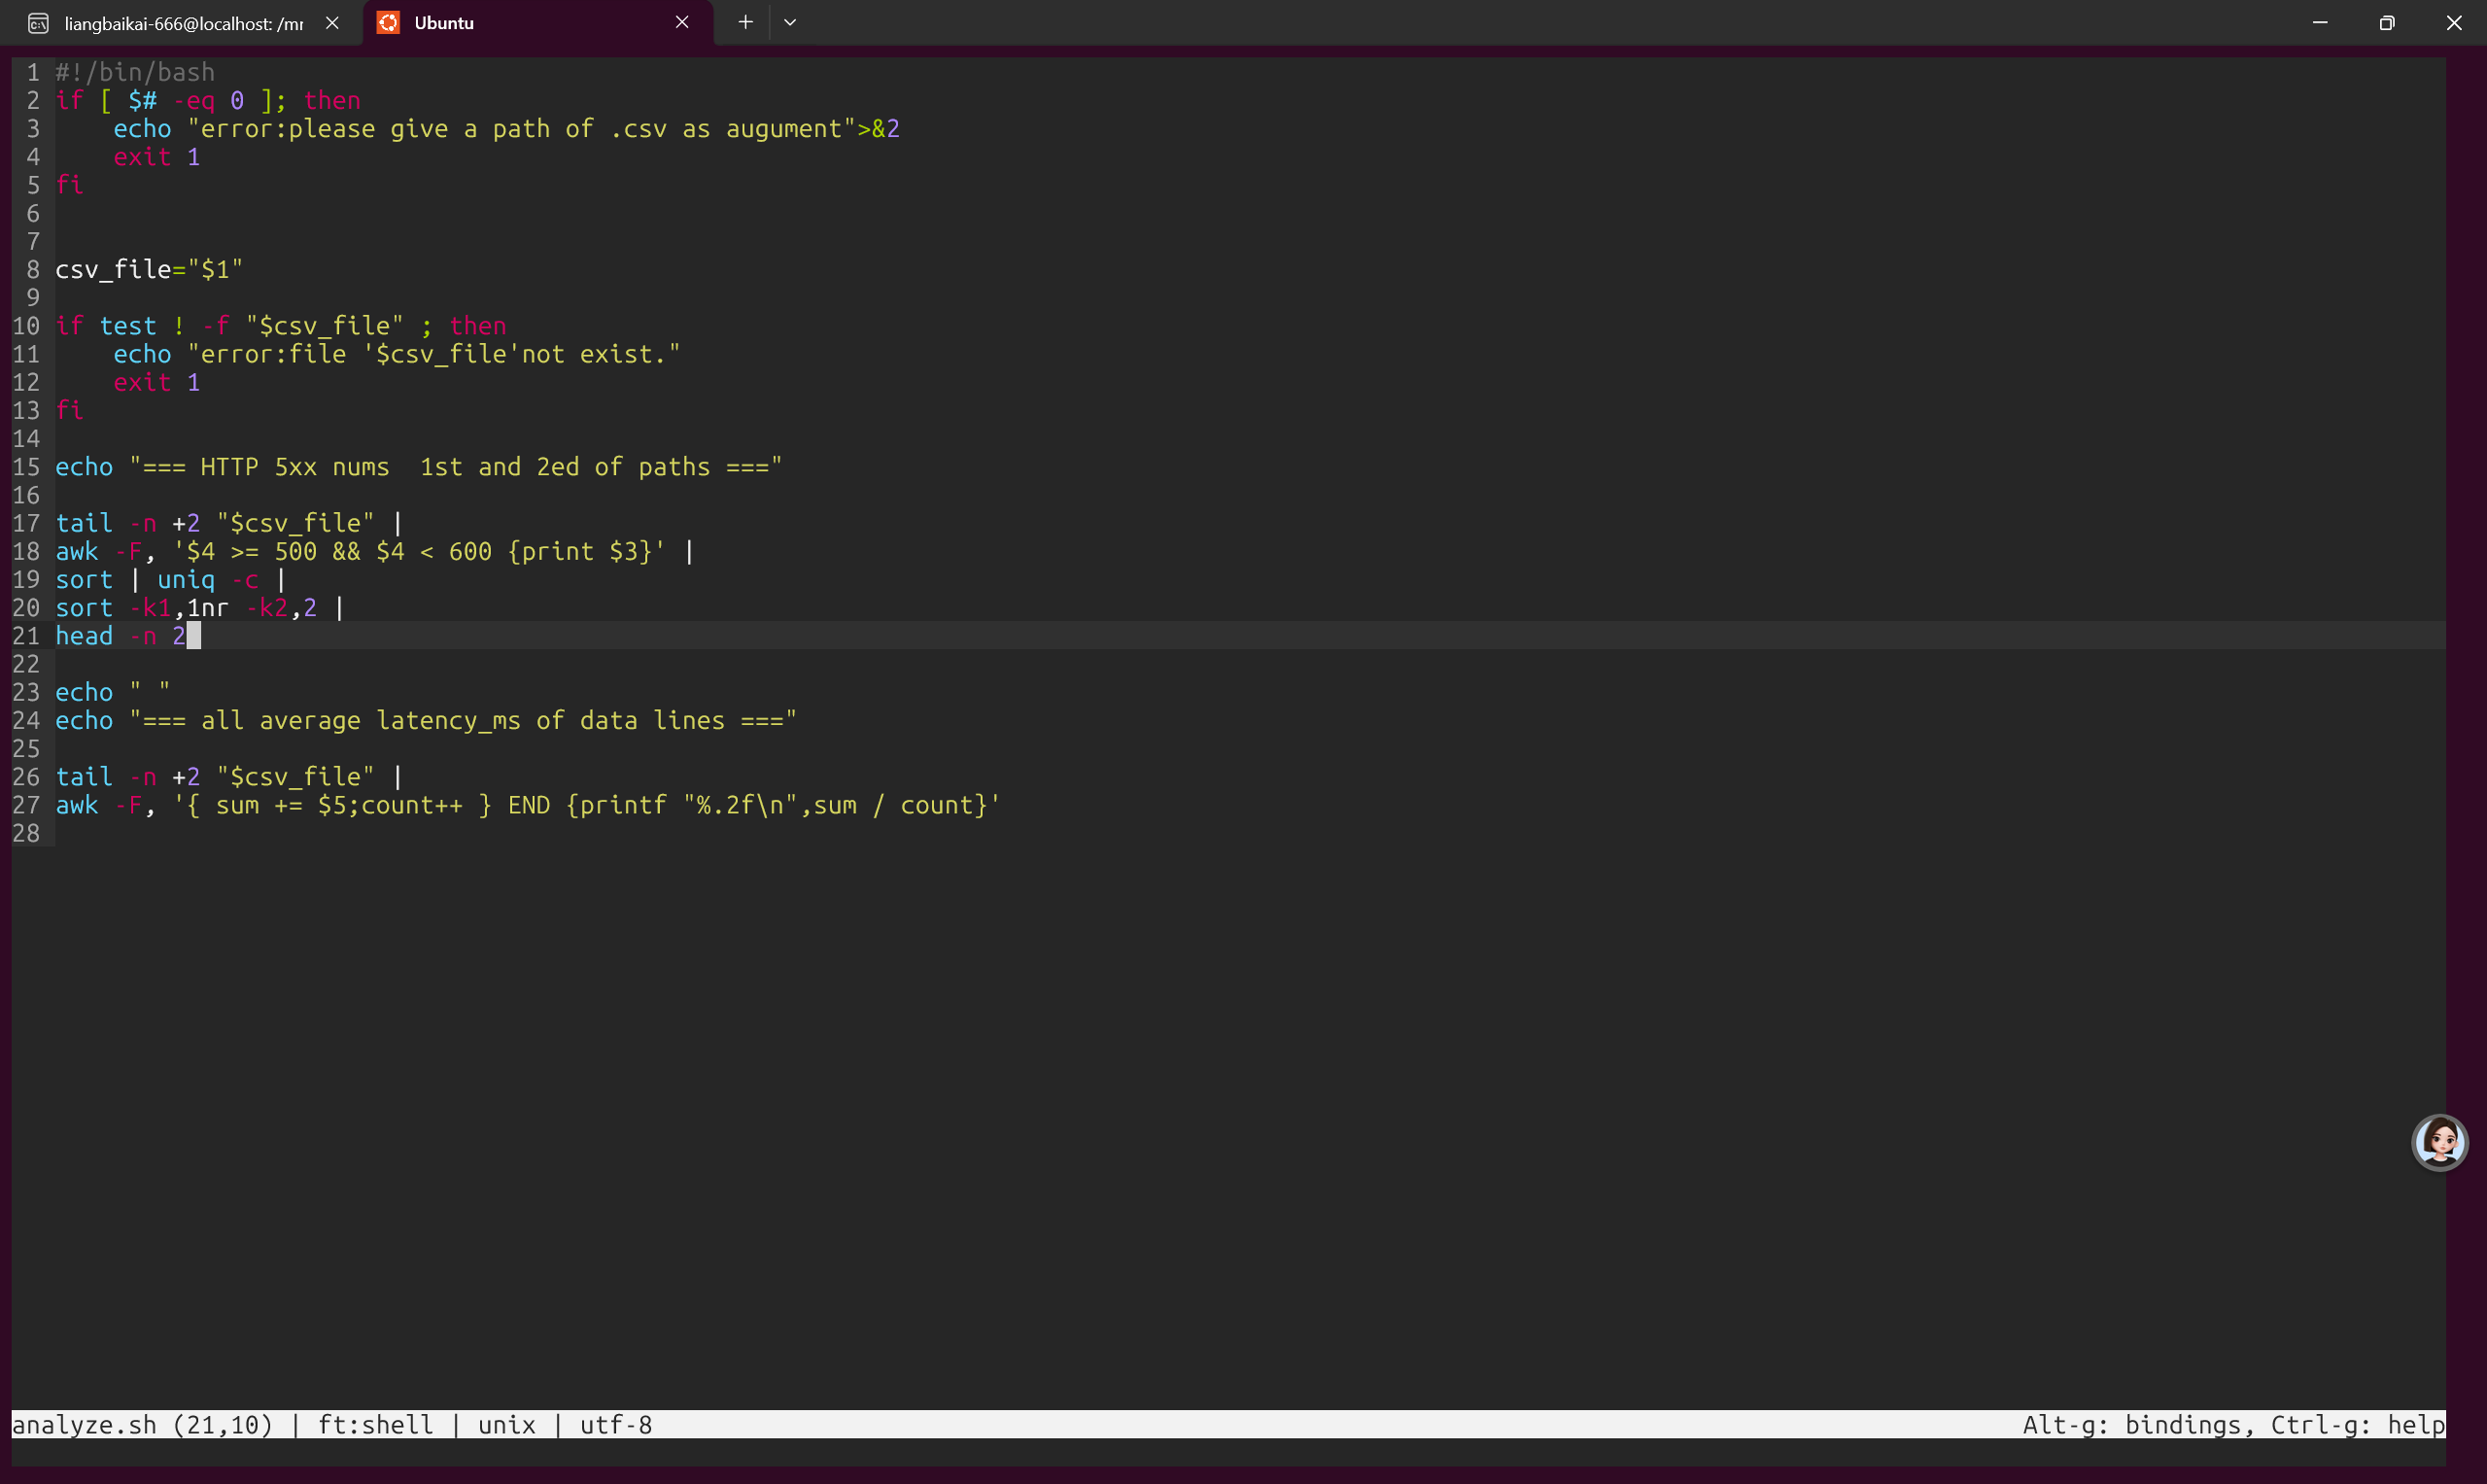
\includegraphics[width=\textwidth]{q02-3.png}
    \caption{最终 \texttt{analyze.sh} 完整代码（micro 编辑器）}
    \label{fig:q02c}
  \end{subfigure}
  \caption{第 2 题：随机访问日志统计全过程截图}
  \label{fig:q02}
\end{figure}

% ============================================================
\section{第 3 题：制造、解决并解释一次合并冲突}

\subsection{操作过程}

从零创建仓库，在 \texttt{main} 完成初始提交后，
\texttt{feature-a} 与 \texttt{feature-b} 均基于初始提交
修改同一文件 \texttt{config.txt} 的同一行，为冲突做准备。
分支操作全部使用 \texttt{git switch} 命令：

\begin{lstlisting}[language=bash]
# 1. 创建目录并初始化仓库(main 为默认分支)
git init q03
cd q03
git init -b main

# 2. 在 main 创建 config.txt 并初始提交
echo "mode=normal" > config.txt
git add config.txt
git commit -m "Initial commit: mode=normal"

# 3. feature-a: 基于初始提交, 改为 mode=safe 并提交
git switch -c feature-a          # 等价于 git checkout -b feature-a
echo "mode=safe" > config.txt
git add config.txt
git commit -m "feature-a: change to mode=safe"

# 4. 回到 main, 从初始 main 新建 feature-b: 改为 mode=fast 并提交
git switch main
git switch -c feature-b
echo "mode=fast" > config.txt
git add config.txt
git commit -m "feature-b: change to mode=fast"

# 5. 回到 main, 先合并 feature-a(可快进), 再合并 feature-b(产生冲突)
git switch main
git merge feature-a              # fast-forward, 无冲突
git merge feature-b              # CONFLICT (content): Merge conflict in config.txt

# 6. 查看冲突 → 在 micro 中编辑解决 → 提交
micro config.txt                 # 看到冲突标记 <<<<<<< ======= >>>>>>>
git add config.txt
git commit -m "Merge feature-b, resolve conflict: keep mode=safe, add note"

# 7. 确认工作区干净, 查看全部提交历史
git status
git log --all --graph --decorate --oneline
\end{lstlisting}

\subsection{冲突原因与解决}

合并 \texttt{feature-a} 时因可快进（fast-forward，
\texttt{93834e3..553a099}）而顺利完成；随后合并
\texttt{feature-b} 时，两个分支基于同一初始版本
（\texttt{93834e3 Initial commit: mode=normal}）
各自把 \texttt{config.txt} 的同一行改为不同内容
（\texttt{feature-a} 改为 \texttt{mode=safe}，
\texttt{feature-b} 改为 \texttt{mode=fast}），
Git 无法自动决定保留哪一个，于是产生内容冲突。

冲突标记如图~\ref{fig:q03}b 所示，\texttt{micro} 编辑器中可见：

\begin{lstlisting}[numbers=none]
<<<<<<< HEAD
mode=safe
=======
mode=fast
>>>>>>> feature-b
\end{lstlisting}

在 \texttt{micro} 中删除冲突标记，保留 \texttt{mode=safe}，
并按要求另加一行 \texttt{note=reviewed}，
最终 \texttt{config.txt} 内容为：

\begin{lstlisting}[numbers=none]
mode=safe
note=reviewed
\end{lstlisting}

经 \texttt{git add config.txt} 与提交后，
\texttt{git status} 显示 \texttt{nothing to commit, working tree clean}，
工作区干净。

\subsection{提交历史}

运行 \texttt{git log --all --graph --decorate --oneline}，
可以看到 \texttt{main}、\texttt{feature-a}、\texttt{feature-b}
三个分支的分叉与最终合并。提交历史为：

\begin{lstlisting}[numbers=none]
* 230205d (HEAD -> main) Merge feature-b, resolve conflict: keep mode=safe, add note
|\
| * 3f8f7d1 (feature-b) feature-b: change to mode=fast
|/
| * 553a099 (feature-a) feature-a: change to mode=safe
|/
* 93834e3 Initial commit: mode=normal
\end{lstlisting}

完整过程如图~\ref{fig:q03} 所示。

\begin{figure}[htbp]
  \centering
  \begin{subfigure}[b]{0.98\textwidth}
    \centering
    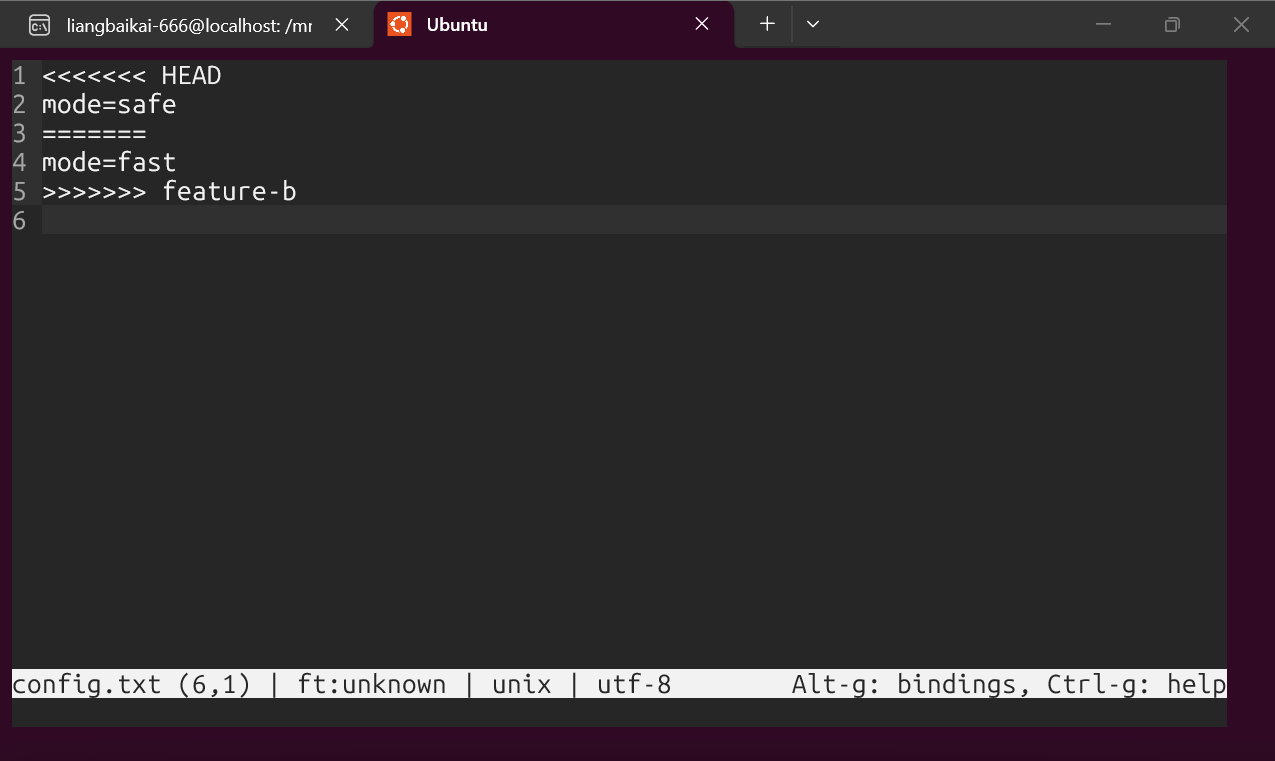
\includegraphics[width=\textwidth]{q03-1.png}
    \caption{完整命令序列：初始化、创建分支、合并产生冲突、解决、提交}
    \label{fig:q03a}
  \end{subfigure}
  \vspace{0.4em}
  \begin{subfigure}[b]{0.98\textwidth}
    \centering
    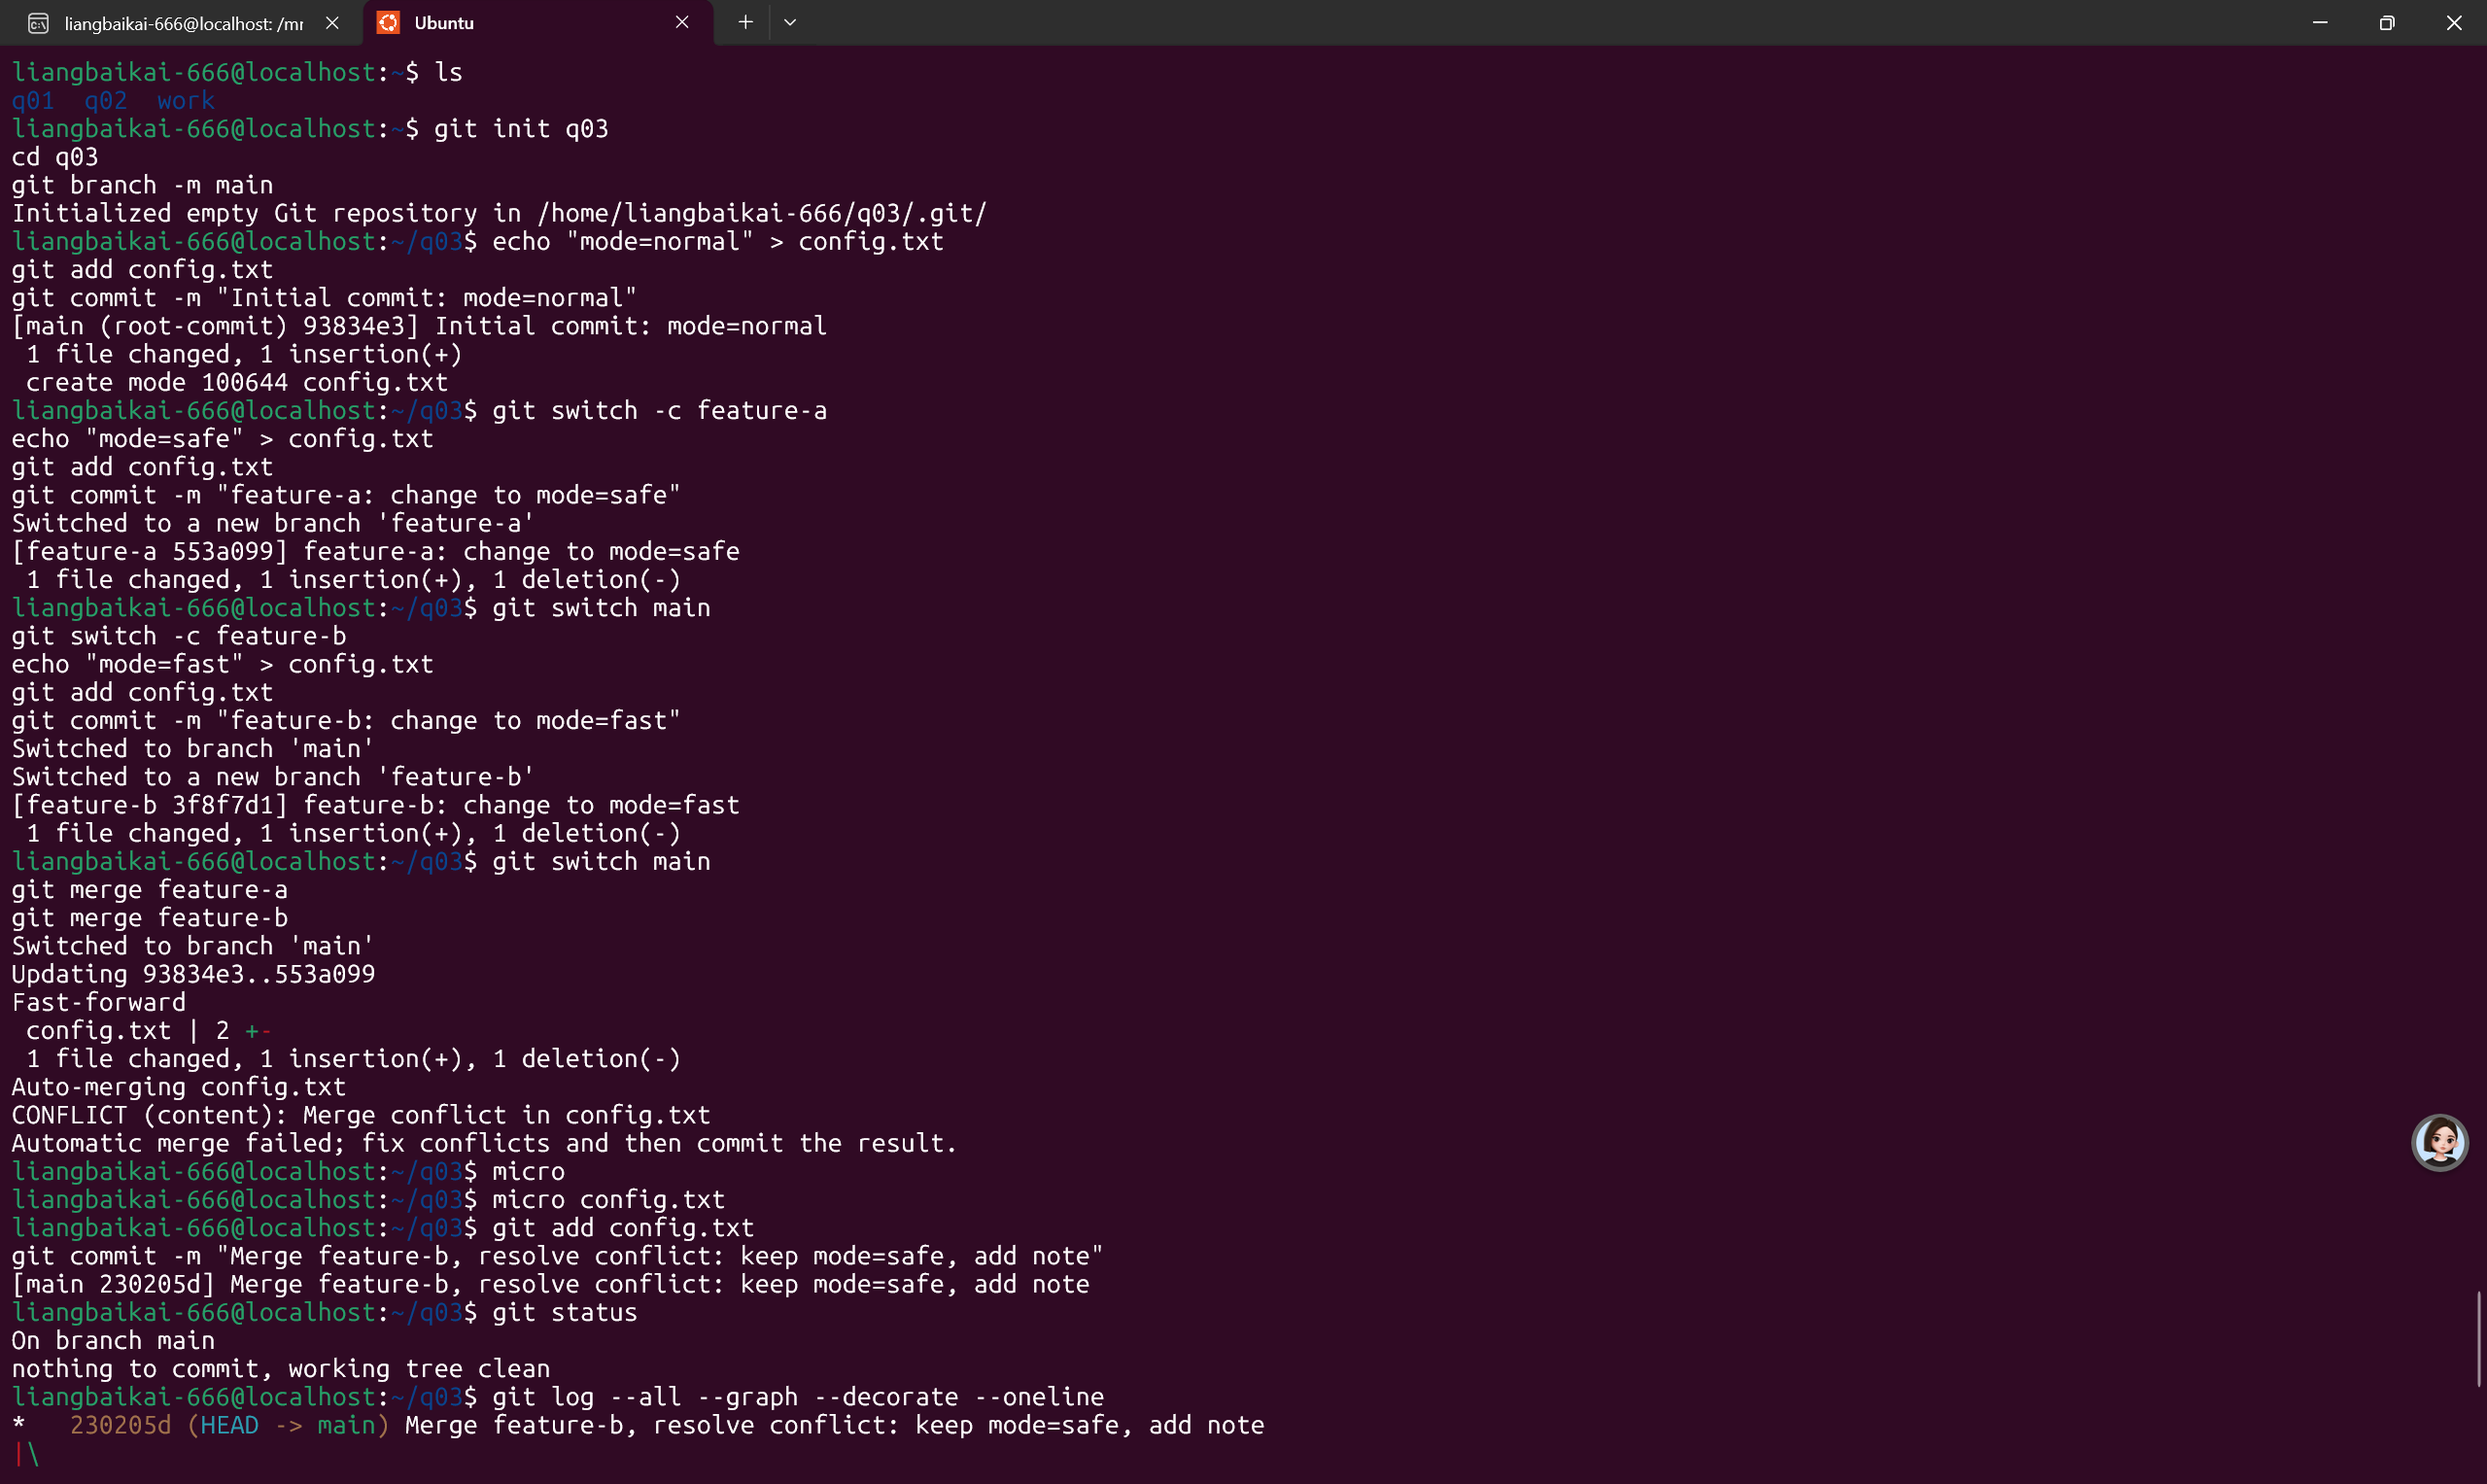
\includegraphics[width=\textwidth]{q03-2.png}
    \caption{\texttt{micro config.txt} 中可见冲突标记
             \texttt{<<<<<<< HEAD / ======= / >>>>>>> feature-b}}
    \label{fig:q03b}
  \end{subfigure}
  \vspace{0.4em}
  \begin{subfigure}[b]{0.98\textwidth}
    \centering
    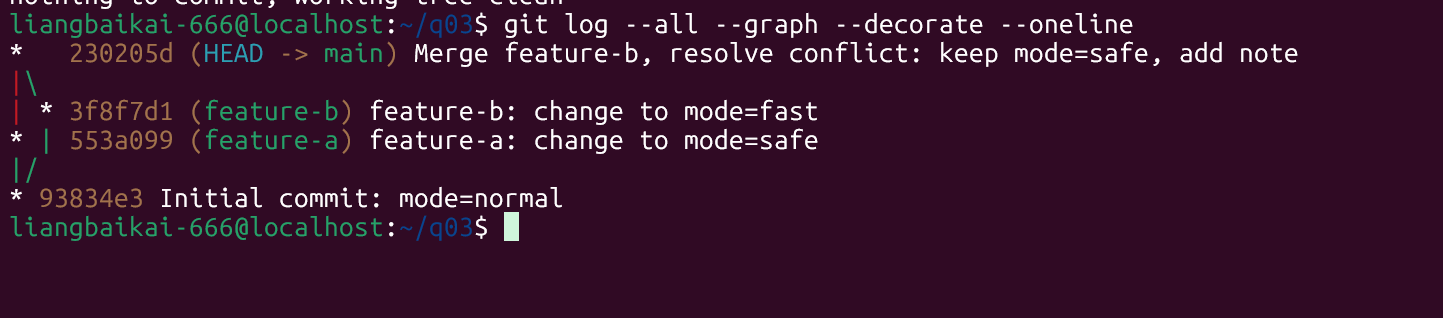
\includegraphics[width=\textwidth]{q03-3.png}
    \caption{\texttt{git log --all --graph --decorate --oneline} 输出}
    \label{fig:q03c}
  \end{subfigure}
  \caption{第 3 题：制造、解决并解释一次合并冲突全过程截图}
  \label{fig:q03}
\end{figure}

% ============================================================
\section{第 4 题：修复并构建一页技术说明}

\subsection{模板补全}

给定模板为 \texttt{article} 文档类加 \texttt{amsmath}，
只需在 \texttt{\textbackslash section\{Result\}} 内补全：
一个带编号公式（\texttt{equation} 环境 + \texttt{\textbackslash label}）、
一个 2 行 2 列表格（\texttt{table} 环境 + \texttt{caption} + \texttt{label}）、
并在正文中用 \texttt{\textbackslash ref} / \texttt{\textbackslash eqref} 交叉引用。
完整 \texttt{report.tex} 如下：

\begin{lstlisting}[language={[LaTeX]TeX}]
\documentclass{article}
\usepackage{amsmath}
\usepackage{booktabs}      % 表格横线
\usepackage{hyperref}     % 超链接与彩色引用

\begin{document}
\title{Tool Report}
\author{王本熙—25020007117}
\maketitle

\section{Result}

% 公式: 带编号 + label, 正文用 \eqref 引用
由式~\eqref{eq:pythagorean} 可得 $a^2 + b^2 = c^2$。

\begin{equation}
  a^2 + b^2 = c^2 \label{eq:pythagorean}
\end{equation}

% 表格: 2 行 2 列 + caption + label, 正文用 \ref 引用
表~\ref{tab:example} 展示了示例数据。

\begin{table}[htbp]
  \centering
  \caption{示例数据表}\label{tab:example}
  \begin{tabular}{cc}
    \toprule
    A & B \\
    \midrule
    1 & 2 \\
    3 & 4 \\
    \bottomrule
  \end{tabular}
\end{table}

\end{document}
\end{lstlisting}

关键点：
\begin{itemize}
  \item \texttt{equation} 环境自动编号，\texttt{\textbackslash label\{eq:pythagorean\}}
        在编译后被 \texttt{\textbackslash eqref} 解析为带括号的编号；
  \item \texttt{table} 浮动体必须加 \texttt{\textbackslash caption} 才能编号，
        \texttt{\textbackslash label} 放在 \texttt{\textbackslash caption} 之后；
  \item \texttt{hyperref} 包让交叉引用变为可点击链接。
\end{itemize}

\subsection{命令行构建}

使用 XeLaTeX 连续编译两遍：第一遍生成 \texttt{.aux}、\texttt{.toc}
等辅助文件并写入 label 的编号，第二遍读取辅助文件解析
\texttt{\textbackslash ref} / \texttt{\textbackslash eqref}，
保证引用不显示 \texttt{??}：

\begin{lstlisting}[language=bash, numbers=none]
cd q04
xelatex report.tex    # 第一遍: 生成辅助文件, 写入 label
xelatex report.tex    # 第二遍: 解析交叉引用, 写入 PDF
\end{lstlisting}

若第一遍后 PDF 中出现 \texttt{式 ??} 或 \texttt{表 ??}，
再运行一遍 \texttt{xelatex} 即可消除。
编译成功后 \texttt{report.pdf} 共 1 页，打开确认：
标题、作者、日期正确，
公式编号为 \textbf{(1)}、表格编号为 \textbf{1}，
正文中的交叉引用均为实际编号而非 \texttt{??}。
最终 PDF 效果如图~\ref{fig:q04} 所示。

\begin{figure}[htbp]
  \centering
  
\includegraphics[width=0.85\textwidth]{q04-1.png}
  \caption{第 4 题：report.pdf 最终效果——式 (1)、表 1 交叉引用正常}
  \label{fig:q04}
\end{figure}

% ============================================================
\section{代码与仓库}

项目已托管至 GitHub：
\url{https://github.com/liangbaikai-666/tool-25020007117}

\subsection{Git 提交记录}

为避免单次全量提交，采用分批提交策略。
\texttt{git log --oneline --graph --decorate --all} 输出如下：

\begin{lstlisting}[language=bash, numbers=none]
* 25c3913 (HEAD -> main, origin/main, origin/HEAD) 统计（ananlyze.sh）脚本
* 71d6ee5 report模板（修改后）
* a3e1519 q01和q03的课后练习
* 2081294 第一次课程的实验报告
* 1c1cc69 Initial commit
\end{lstlisting}

共 5 次提交，作者 \texttt{liangbaikai-666}，
时间集中在 \texttt{Mon Aug 31 14:56 — 15:12 2026 +0800}。
各提交职责清晰：

\begin{itemize}
  \item \texttt{1c1cc69 Initial commit}：仓库初始化；
  \item \texttt{2081294 第一次课程的实验报告}：提交第 1 周实验相关代码；
  \item \texttt{a3e1519 q01和q03的课后练习}：补充 q01 / q03 的课后练习内容；
  \item \texttt{71d6ee5 report模板（修改后）}：更新 \LaTeX{} 实验报告模板；
  \item \texttt{25c3913 统计（ananlyze.sh）脚本}：最终提交 \texttt{analyze.sh} 统计脚本。
\end{itemize}

\begin{figure}[htbp]
  \centering
  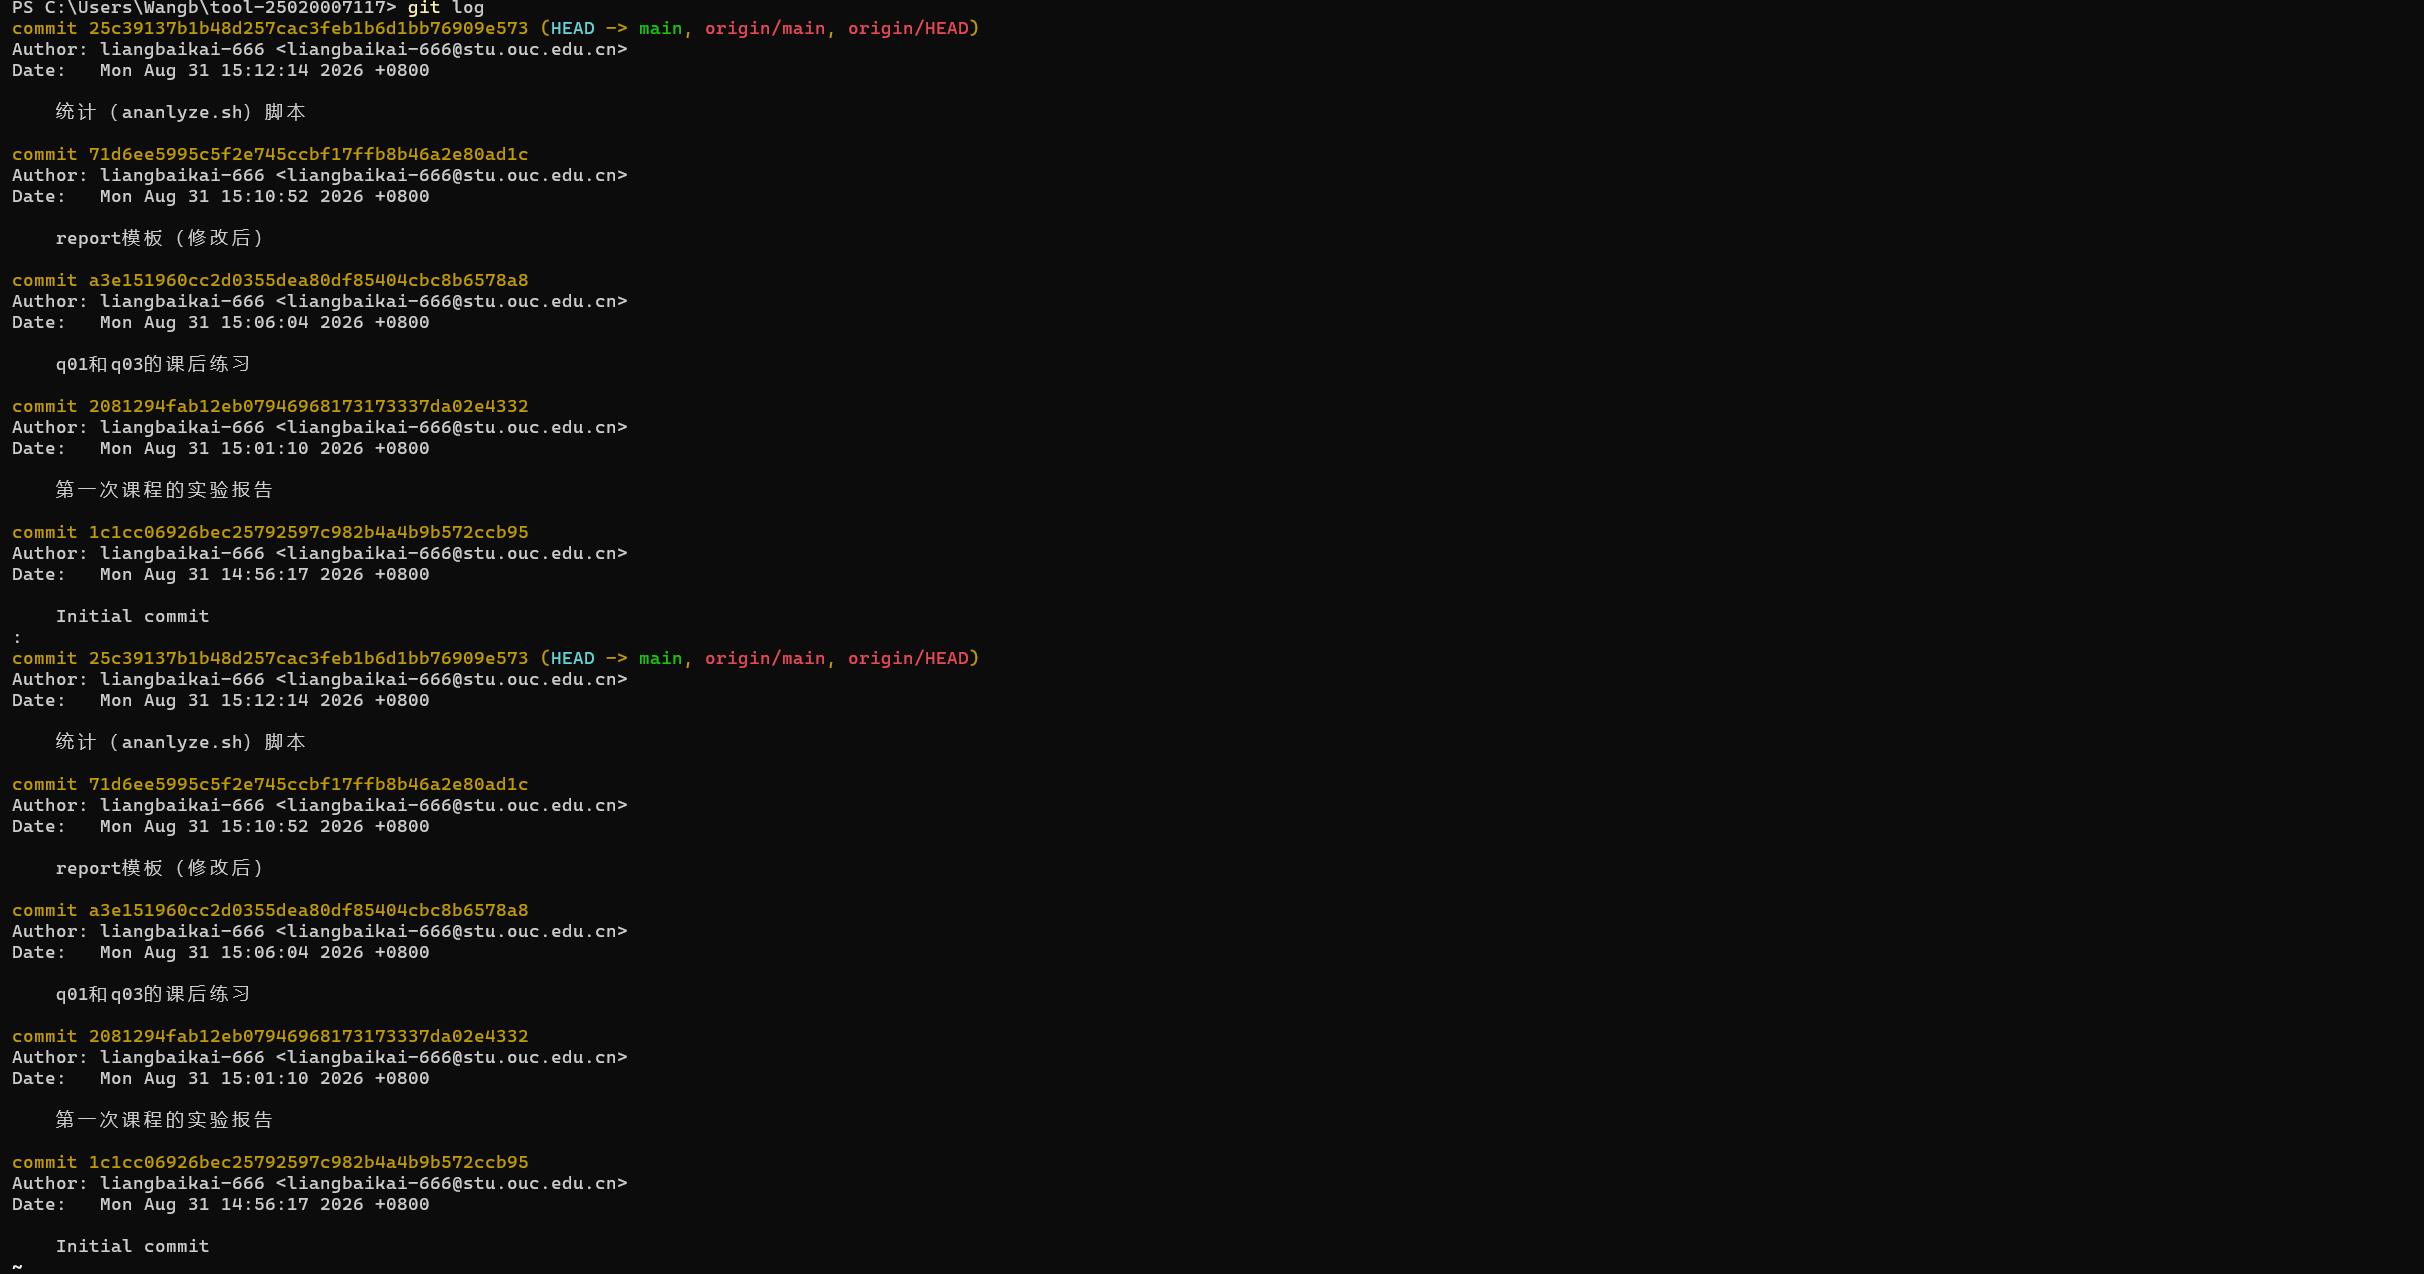
\includegraphics[width=0.9\textwidth]{commit-log.png}
  \caption{Git 提交记录（\texttt{git log} 完整输出）}
  \label{fig:commitlog}
\end{figure}

\subsection{分批提交示例命令}

在 WSL (Ubuntu) 终端中，以 \texttt{q03} 为例展示常见分批提交流程：

\begin{lstlisting}[language=bash]
# 初始化
cd /path/to/project
git init -b main
git remote add origin https://github.com/liangbaikai-666/tool-25020007117.git

# 分批提交(每次只提交相关文件, 避免全量提交)
git add q01/              && git commit -m "feat: q01 shell batch file rename"
git add q02/              && git commit -m "feat: q02 analyze.sh log statistics"
git add q03/              && git commit -m "feat: q03 merge conflict demo"
git add q04/              && git commit -m "feat: q04 latex report with cross-ref"
git add report1.tex       && git commit -m "docs: add week1 experiment report"
git add report1.pdf       && git commit -m "docs: add compiled report1.pdf"

# 推送
git push -u origin main
\end{lstlisting}

% ============================================================
\section{结论}

通过第 1 周实验，完成了四道课上检查题：
（1）使用 Shell 命令完成含空格文件名的批量整理，
通过 \texttt{rsync} 的 \texttt{--include/--exclude} 规则
精准收齐所有 \texttt{.txt}（含空格文件名与隐藏文件），
并按 750/640 设置权限、生成字节数清单；
（2）编写 \texttt{analyze.sh}，以管道串联 \texttt{awk}、\texttt{sort}、
\texttt{head} 统计 5xx 次数前 2 的 path 与平均延迟，
并规范处理错误流与退出码；
（3）在 Git 中主动制造并解决一次合并冲突，
理解了冲突产生的条件与解决流程；
（4）在 \LaTeX{} 模板中加入带编号公式与表格并完成交叉引用，
从命令行编译生成无 \texttt{??} 的 PDF。
实验达到预期目标。

\end{document}
